
\begin{figure}
\begin{minted}{python}
    # This program adds two numbers
    num1 = 1.5
    num2 = 6.3
    # Add two numbers
    sum = num1 + num2
    # Display the sum
    print('The sum of {0} and {1} is {2}'.format(num1, num2, sum))
\end{minted}
\caption{Simplest use of PHASM surrogate API}
\end{figure}






\begin{block}{Strategic goals}

Interactive tool for empirical testing of surrogate models
Automate as much as possible, but not everything
Similar to a debugger: pause execution of a (compiled) program, present the user with a prompt. From here the user can profile a function, rewrite the binary to replace a function with a surrogate, tune the surrogate’s hyperparameters, etc.
Same process as by hand, except orders of magnitude faster
\end{block}

\begin{figure}
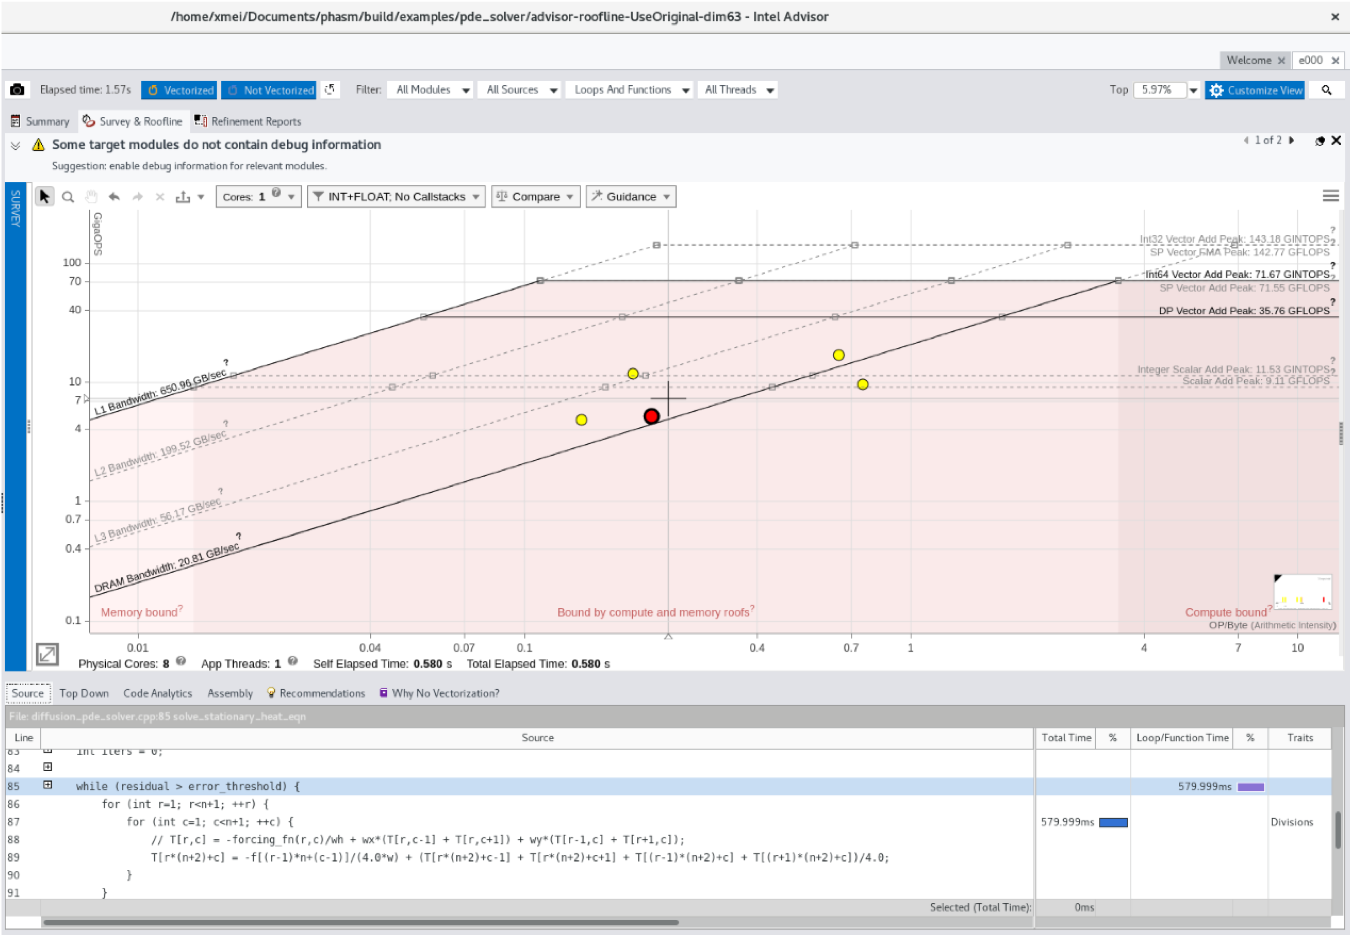
\includegraphics[width=0.8\linewidth]{roofline.png}
\caption{Roofline analysis of a compute kernel}
\end{figure}

%----------------------------------------------------------------------------------------
%   ADDITIONAL INFORMATION
%----------------------------------------------------------------------------------------

\begin{block}{Next steps}

\begin{description}
\item[Multiple ML backends]\ Rearchitect the Surrogate API to support multiple ML frameworks via dynamically loaded backends, similar to how GlueX+JANA uses plugins.

\item[MLFlow integration]\ MLFlow is a model repository that handles versioning, annotating, and sharing of trained machine learning models. It is a research priority of JLab’s data science department.

\item[Static analysis]\ Experiment with performing a static code analysis for model variable discovery instead, using ROSE or LLVM/clang. 

\item[Validate using Geant4] Use PHASM to demonstrate effective subevent-level parallelism within Geant4. Create a surrogate for a calorimeter detector simulation kernel. This kernel has already been calculated to perform well under GPU offloading, but no CUDA port has been written.

\end{description}

\end{block}


\begin{block}{References}
\begin{itemize}
\item Code: \href{http://www.github.com/nathanwbrei/phasm}{http://www.github.com/nathanwbrei/phasm}
\item Wiki: \href{https://wiki.jlab.org/epsciwiki/index.php/AI_Surrogate_Models_LDRD}{https://wiki.jlab.org/epsciwiki/index.php/AI_Surrogate_Models_LDRD}
\item Email: \href{mailto:nbrei@jlab.org}{nbrei@jlab.org}
\end{itemize}
\end{block}
